
On donne ci-dessous le patron d’un cube avec divers motifs sur chacune des faces.\\
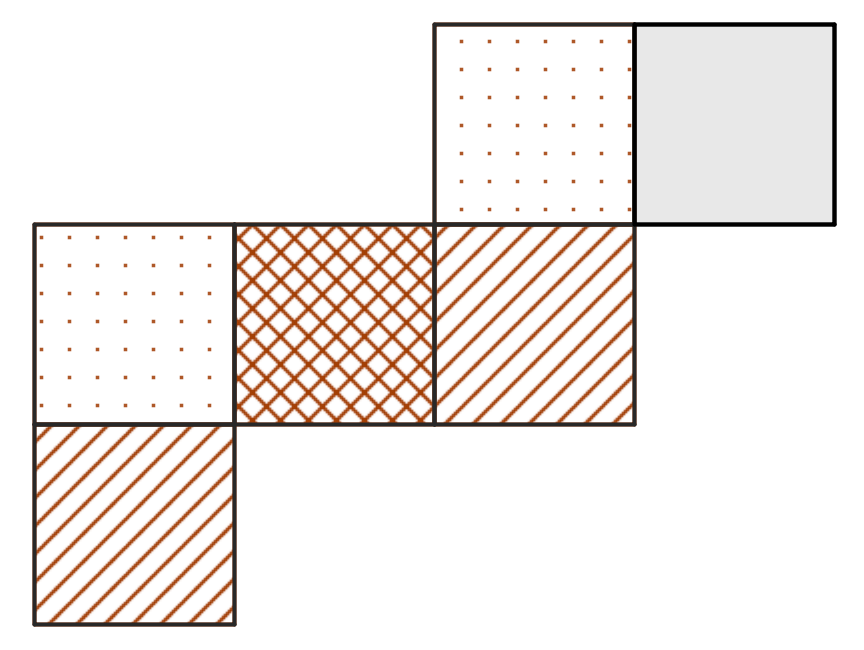
\includegraphics[scale=0.4]{RepS-flash3}

\medskip
 
Sur les représentations en perspective ci-dessous, compléter les motifs sur chacune des faces
visibles (on ne tiendra pas compte de l’orientation des hachures sur les faces) afin d’obtenir
trois vues en perspective différentes du cube initial.
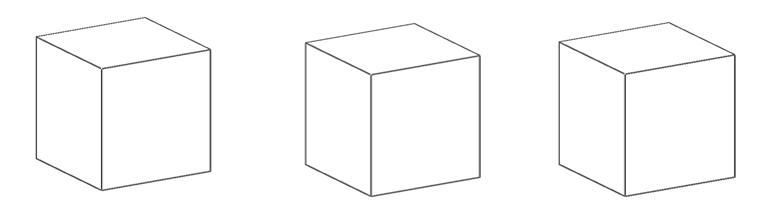
\includegraphics[scale=0.7]{RepS-flash3b}

